\documentclass[12pt]{article}

\usepackage[a4paper,left=0.82in,right=0.82in,top=0.9in,bottom=0.95in]{geometry}
\usepackage[T1]{fontenc}
\usepackage[utf8]{inputenc}
\usepackage{lmodern}
\usepackage{amsmath,amssymb,amsthm,mathtools}
\usepackage{booktabs}
\usepackage{array}
\usepackage{microtype}
\usepackage{xcolor}
\usepackage{hyperref}
\usepackage{enumitem}
\usepackage{setspace}

\hypersetup{
  colorlinks=true,
  linkcolor=blue!55!black,
  citecolor=blue!55!black,
  urlcolor=blue!55!black
}

\setstretch{1.055}
\setlength{\parindent}{0pt}
\setlength{\parskip}{0.52em}
\setlist[itemize]{topsep=0.25em,itemsep=0.15em}
\setlist[enumerate]{topsep=0.25em,itemsep=0.15em}

\theoremstyle{plain}
\newtheorem{theorem}{Theorem}
\newtheorem{lemma}[theorem]{Lemma}
\newtheorem{proposition}[theorem]{Proposition}
\newtheorem{corollary}[theorem]{Corollary}
\theoremstyle{definition}
\newtheorem{definition}[theorem]{Definition}
\theoremstyle{remark}
\newtheorem{remark}[theorem]{Remark}

\newcommand{\Lop}{\mathcal L}
\newcommand{\binomtwo}[1]{\binom{#1}{2}}
\newcommand{\floor}[1]{\left\lfloor #1\right\rfloor}
\newcommand{\ceil}[1]{\left\lceil #1\right\rceil}
\newcommand{\supp}{\operatorname{supp}}

\begin{document}

\title{%
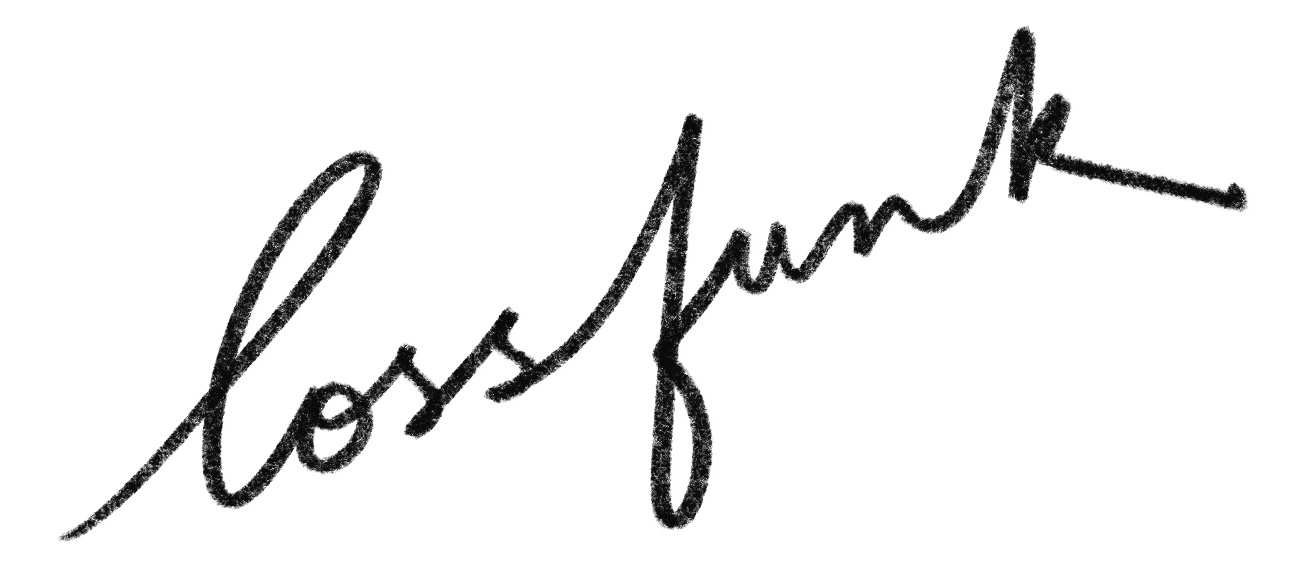
\includegraphics[width=0.33\linewidth]{lossfunk-logo.jpg}\\[0.85cm]
A Colored Turan Proof of the Lollipop Formula}
\author{Siddhartha Mahajan \and Paras Chopra}
\date{\today}
\maketitle

\begin{abstract}
Let \(a_{\Lop}(n)\) be the maximum number of connected regions into which
\(n\) lollipops can divide the plane.  We prove, from Paulsen's two geometric
obstructions, the exact four-cluster formula
\[
  a_{\Lop}(n)=4\binom n2+S(n)+n+1,
\]
where
\[
  S(n)=\max_{a+b+c+d=n,\;0\le a\le b\le c\le d}
  \left(3\sum_{1\le i<j\le4}m_i m_j-2ab\right),
  \qquad (m_1,m_2,m_3,m_4)=(a,b,c,d).
\]
The proof is entirely combinatorial after the geometric reduction.  It uses a
colored Zykov symmetrization, a weighted blocker lemma, and an exact
\(3\times4\) matrix inequality.  The matrix inequality is proved by support
compression: alternating four-edge path compressions and double-star
compressions reduce every integer matrix to star-forest normal form, where the
efficient degree pattern is \(K_{1,2}\cup K_2\cup K_2\).  This also explains
the asymptotic cluster proportions
\[
  \frac{3}{16},\frac{3}{16},\frac{5}{16},\frac{5}{16}.
\]
\end{abstract}

\section{The formula}

A \emph{lollipop} is a circle together with a half-line attached at one point
of the circle and extending radially outward.  We assume arrangements are
generic: there are no tangencies, no triple intersection points, and no
intersection occurs at an anchor point.  This entails no loss for a maximum,
since a non-generic arrangement can be perturbed without decreasing the number
of regions.

Let \(C\) be the total number of crossings between distinct lollipops.  Adding
one generic lollipop with \(k\) crossings increases the number of regions by
\(k+1\), and hence
\begin{equation}\label{eq:regions}
  \#\hbox{regions}=C+n+1.
\end{equation}
Thus the problem is to maximize \(C\).

For \(n\ge0\), define
\begin{equation}\label{eq:Sdef}
  S(n)=\max_{a+b+c+d=n,\;0\le a\le b\le c\le d}
  \left(3\sum_{1\le i<j\le4}m_i m_j-2ab\right),
  \qquad (m_1,m_2,m_3,m_4)=(a,b,c,d).
\end{equation}
Equivalently, for a fixed multiset of four cluster sizes, the penalized pair is
the pair with smallest product, i.e. the two smallest clusters.

\begin{theorem}\label{thm:lollipop-formula}
For every \(n\ge0\),
\begin{equation}\label{eq:main-formula}
  a_{\Lop}(n)=4\binom n2+S(n)+n+1.
\end{equation}
\end{theorem}

The first values obtained from \eqref{eq:main-formula} are
\[
\begin{gathered}
1,2,10,25,45,71,104,142,186,237,294,356,425,500,580,667,\\
761,859,964,1076,1193,1316,1446,1581,1722,1870,2024,2183,\\
2349,2521,2698,2882,3073.
\end{gathered}
\]

\section{Geometric input and the two-graph reduction}

We use Paulsen's terminology.  A pair of lollipops is \emph{close} if the
angle between the two stem directions is at most \(90^\circ\).  A pair is
\emph{intriguing} if the two circles either do not meet, or meet at angle at
most \(90^\circ\), after orienting the two circles in the same direction.

The following geometric facts are due to Cutler--Karlsson--Sloane and Paulsen.
The present paper is a self-contained proof of the combinatorial extremal step
that follows from these facts.

\begin{lemma}[geometric lollipop input]\label{lem:geometry}
For a generic pair of lollipops:
\begin{enumerate}[label=(\roman*)]
  \item a close pair has at most \(5\) crossings;
  \item an intriguing pair has at most \(5\) crossings;
  \item a pair that is both close and intriguing has at most \(4\) crossings.
\end{enumerate}
Furthermore, among any four lollipops there is a close pair, and among any five
lollipops there is an intriguing pair.
\end{lemma}

Given an arrangement of \(n\) lollipops, define graphs \(D,E\) on the same
vertex set by
\[
  ij\in D\quad\Longleftrightarrow\quad L_i,L_j\hbox{ are not close},
\]
\[
  ij\in E\quad\Longleftrightarrow\quad L_i,L_j\hbox{ are not intriguing}.
\]
By Lemma \ref{lem:geometry},
\begin{equation}\label{eq:forbidden-DE}
  D\hbox{ is }K_4\hbox{-free},\qquad E\hbox{ is }K_5\hbox{-free}.
\end{equation}
For a pair \(ij\), Lemma \ref{lem:geometry} gives the pointwise estimate
\begin{equation}\label{eq:pair-weight}
  c_{ij}\le
  4+\mathbf 1_{ij\in D}+\mathbf 1_{ij\in E}+\mathbf 1_{ij\in D\cap E}.
\end{equation}
Therefore
\begin{equation}\label{eq:two-graph-bound}
  C\le 4\binom n2+\sigma(D,E),
  \qquad
  \sigma(D,E):=|D|+|E|+|D\cap E|.
\end{equation}
Theorem \ref{thm:lollipop-formula} is now reduced to the following colored
Turan theorem.

\begin{theorem}[colored Turan theorem]\label{thm:colored-turan}
If \(D\) is \(K_4\)-free and \(E\) is \(K_5\)-free on the same \(n\)-vertex
set, then
\begin{equation}\label{eq:sigma-upper}
  \sigma(D,E)\le S(n).
\end{equation}
\end{theorem}

The proof occupies Sections \ref{sec:zykov}--\ref{sec:matrix}.  The lower
construction is given in Section \ref{sec:lower}; together with
\eqref{eq:regions} and \eqref{eq:two-graph-bound}, it proves Theorem
\ref{thm:lollipop-formula}.

\section{Colored Zykov symmetrization}\label{sec:zykov}

Color every unordered pair of vertices with one of four colors:
\[
  0: \hbox{neither }D\hbox{ nor }E,
  \qquad
  A: E\hbox{-only},
\]
\[
  B: D\hbox{-only},
  \qquad
  X: D\cap E.
\]
These colors have weights
\[
  w(0)=0,\\quad w(A)=1,
  \quad w(B)=1,
  \quad w(X)=3,
\]
so that \(\sigma(D,E)\) is the total color-weight.

\begin{lemma}[colored Zykov reduction]\label{lem:zykov}
An extremal pair \((D,E)\) for \(\sigma\) may be chosen as a blow-up of a
complete colored quotient: the vertex set is partitioned into classes
\(V_1,\ldots,V_k\), every pair inside one class has color \(0\), and every pair
between two distinct classes has one fixed color from \(\{A,B,X\}\).  In
particular, there are no color-\(0\) pairs between distinct classes.
\end{lemma}

\begin{proof}
Suppose \(uv\) has color \(0\).  Let \(d_w(v)\) be the total color-weight from
\(v\) to all vertices other than \(u,v\).  If \(d_w(u)\le d_w(v)\), replace
\(u\) by a clone of \(v\): for every \(z\ne u,v\), give \(uz\) the same color
as \(vz\), while keeping \(uv\) color \(0\).  This operation changes \(\sigma\)
by \(d_w(v)-d_w(u)\ge0\).

It cannot create a \(K_4\) in \(D\).  Indeed, a new \(D\)-clique using the
clone \(u\) and not \(v\) corresponds to the same clique with \(v\) in place of
\(u\), while a clique using both \(u\) and \(v\) is impossible because \(uv\) is
not a \(D\)-edge.  The same argument forbids creation of a \(K_5\) in \(E\).
Thus the operation preserves \eqref{eq:forbidden-DE} and does not decrease
\(\sigma\).

Repeating this operation, with the standard tie-breaker of maximizing the sum
of squares of the resulting clone-class sizes among all extremal pairs,
terminates in a configuration in which color-\(0\) is an equivalence relation
whose classes are twins.  Between two distinct equivalence classes all pairs
have one nonzero color; otherwise a further cloning or tie-breaking step would
be possible.  This is the claimed quotient form.
\end{proof}

Let the quotient class sizes be \(x_1,\ldots,x_k\), with
\(\sum_i x_i=n\), and put
\[
  Q=\sum_i x_i^2.
\]
Let
\[
  a=\sum_{ij\in A}x_i x_j,
  \qquad
  b=\sum_{ij\in B}x_i x_j,
\]
where \(A\) and \(B\) now also denote the graphs of \(A\)-colored and
\(B\)-colored quotient edges.  The total cross-class mass is
\[
  P=\sum_{i<j}x_i x_j=\frac{n^2-Q}{2}.
\]
Since \(X\)-edges have weight \(3\), while \(A\)- and \(B\)-edges have weight
\(1\),
\begin{equation}\label{eq:sigma-quotient}
  \sigma=3P-2a-2b=\frac32(n^2-Q)-2a-2b.
\end{equation}

The forbidden cliques translate into blocker conditions.  Since
\(D\) consists of colors \(B\cup X\), every four quotient vertices contain an
\(A\)-edge; otherwise they form a \(K_4\) in \(D\).  Thus
\begin{equation}\label{eq:alphaA}
  \alpha(A)\le3.
\end{equation}
Similarly, since \(E\) consists of colors \(A\cup X\),
\begin{equation}\label{eq:alphaB}
  \alpha(B)\le4.
\end{equation}

\section{The weighted blocker lemma}\label{sec:blocker}

For nonnegative integer weights \(x_1,\ldots,x_k\) with total \(n\), define
\(Q=\sum_i x_i^2\).  If \(G\) is a graph on \([k]\), write
\[
  w(G)=\sum_{ij\in E(G)}x_i x_j.
\]

For \(r\ge1\), let
\[
  \rho_r(x)=\min_{\mathcal P}\sum_{P\in\mathcal P}
  \left(\sum_{i\in P}x_i\right)^2,
\]
where the minimum is over all partitions of \([k]\) into \(r\) possibly empty
parts.

\begin{lemma}[weighted Turan theorem]\label{lem:weighted-turan}
If \(G\) is \(K_{r+1}\)-free, then
\begin{equation}\label{eq:weighted-turan}
  w(G)\le\frac12\bigl(n^2-\rho_r(x)\bigr).
\end{equation}
\end{lemma}

\begin{proof}
The usual Zykov symmetrization works with vertex weights: if two nonadjacent
vertices have different weighted neighborhoods, clone the smaller weighted
neighborhood to the larger one.  This preserves \(K_{r+1}\)-freeness and does
not decrease \(w(G)\).  An extremal weighted graph is therefore a complete
multipartite graph with at most \(r\) parts.  For a partition with part weights
\(s_1,\ldots,s_r\), its edge weight is
\[
  \sum_{i<j}s_i s_j=\frac12\left(n^2-\sum_i s_i^2\right),
\]
which is maximized exactly when \(\sum_i s_i^2\) is minimized.
\end{proof}

Define
\begin{equation}\label{eq:Mdef}
  M(n)=\min_{a+b+c+d=n,\;a,b,c,d\in\mathbb Z_{\ge0}}
  \left[\frac32(a^2+b^2+c^2+d^2)+2ab\right].
\end{equation}
Since
\[
  \frac32n^2-
  \left[\frac32(a^2+b^2+c^2+d^2)+2ab\right]
  =3\sum_{i<j}m_i m_j-2ab,
\]
where \((m_1,m_2,m_3,m_4)=(a,b,c,d)\), and since the two variables in the
penalized product may be labelled as the two smallest cluster sizes, the
definitions imply
\begin{equation}\label{eq:S-M}
  S(n)=\frac32 n^2-M(n).
\end{equation}

\begin{lemma}[weighted blocker lemma]\label{lem:blocker}
Let \(A,B\) be graphs on \([k]\) with \(\alpha(A)\le3\) and
\(\alpha(B)\le4\).  With the notation above,
\begin{equation}\label{eq:blocker}
  \frac32Q+2w(A)+2w(B)\ge M(n).
\end{equation}
\end{lemma}

\begin{proof}
The complement of \(A\) is \(K_4\)-free.  By Lemma \ref{lem:weighted-turan},
\[
  \frac12(n^2-Q)-w(A)
  \le \frac12(n^2-\rho_3(x)),
\]
and hence
\begin{equation}\label{eq:a-lower}
  w(A)\ge\frac12(\rho_3(x)-Q).
\end{equation}
Likewise, the complement of \(B\) is \(K_5\)-free, so
\begin{equation}\label{eq:b-lower}
  w(B)\ge\frac12(\rho_4(x)-Q).
\end{equation}
Combining \eqref{eq:a-lower} and \eqref{eq:b-lower},
\begin{equation}\label{eq:rho-bound}
  \frac32Q+2w(A)+2w(B)
  \ge \rho_3(x)+\rho_4(x)-\frac12Q.
\end{equation}

Choose partitions attaining \(\rho_3(x)\) and \(\rho_4(x)\), and intersect
them.  This gives a \(3\times4\) nonnegative integer matrix
\(U=(u_{ij})\), where \(u_{ij}\) is the total weight lying in the \(i\)-th
part of the \(3\)-partition and the \(j\)-th part of the \(4\)-partition.
Let
\[
  r_i=\sum_j u_{ij},\qquad c_j=\sum_i u_{ij}.
\]
Then
\[
  \rho_3(x)=\sum_i r_i^2,
  \qquad
  \rho_4(x)=\sum_j c_j^2.
\]
Also
\[
  Q=\sum_\ell x_\ell^2\le \sum_{i,j}u_{ij}^2,
\]
because squaring after grouping can only increase the sum of squares.  Thus
\eqref{eq:rho-bound} gives
\[
  \frac32Q+2w(A)+2w(B)
  \ge
  \sum_i r_i^2+
  \sum_j c_j^2-\frac12\sum_{i,j}u_{ij}^2.
\]
The right side is at least \(M(n)\) by the matrix theorem proved in
Section \ref{sec:matrix}.
\end{proof}

We now prove Theorem \ref{thm:colored-turan}, assuming the matrix theorem for a
moment.

\begin{proof}[Proof of Theorem \ref{thm:colored-turan}]
By Lemma \ref{lem:zykov}, assume \((D,E)\) is in quotient form.  Then
\eqref{eq:alphaA} and \eqref{eq:alphaB} allow Lemma \ref{lem:blocker}, so
\[
  \frac32Q+2a+2b\ge M(n).
\]
Using \eqref{eq:sigma-quotient},
\[
  \sigma
  =\frac32n^2-\left(\frac32Q+2a+2b\right)
  \le \frac32n^2-M(n)=S(n),
\]
by \eqref{eq:S-M}.  This proves \eqref{eq:sigma-upper}.
\end{proof}

\section{The \texorpdfstring{\(3\times4\)}{3 x 4} matrix theorem}\label{sec:matrix}

For a \(3\times4\) nonnegative integer matrix \(U=(u_{ij})\) with total sum
\(n\), row sums \(r_i\), and column sums \(c_j\), put
\begin{equation}\label{eq:Fdef}
  F(U)=\sum_{i=1}^3 r_i^2+
        \sum_{j=1}^4 c_j^2-\frac12\sum_{i,j}u_{ij}^2.
\end{equation}

\begin{theorem}[matrix theorem]\label{thm:matrix}
For every \(3\times4\) nonnegative integer matrix \(U\) of total sum \(n\),
\begin{equation}\label{eq:matrix-theorem}
  F(U)\ge M(n).
\end{equation}
\end{theorem}

The proof is the main technical point.  Think of the positive entries of
\(U\) as edge masses on the bipartite graph \(K_{3,4}\), whose left vertices
are the rows and whose right vertices are the columns.  If two positive cells
share a row or a column, call the corresponding edges adjacent.  Expanding
\eqref{eq:Fdef} gives
\begin{equation}\label{eq:F-edge}
  F(U)=\frac32\sum_e u_e^2+2\sum_{e\sim f}u_eu_f.
\end{equation}

\subsection*{Compression to a star forest}

The next lemma is the normal-form step needed below: every matrix can be
compressed to a star forest without increasing \(F\).  Equality may occur during
compression, so the conclusion concerns the compressed matrix rather than the
original support.

\begin{lemma}[support compression]\label{lem:compression}
For every nonnegative integer matrix \(U\), there is a nonnegative integer
matrix \(U'\) with the same total sum such that
\[
  F(U')\le F(U)
\]
and the support graph of \(U'\) is a forest whose connected components are
stars.
\end{lemma}

\begin{proof}
First remove cycles.  If the support contains a cycle, add \(\varepsilon\) and
\(-\varepsilon\) alternately around the cycle.  Row sums and column sums, and
therefore the first two terms of \eqref{eq:Fdef}, remain fixed.  The final
term \(-\frac12\sum u_{ij}^2\) is a concave quadratic in \(\varepsilon\), so one
endpoint of the maximal integer interval of allowed \(\varepsilon\)'s does not
increase \(F\) and makes at least one entry zero.  Repeating leaves a forest.

Now suppose a tree component has diameter at least \(4\).  Choose four
consecutive edges on a path in that component, with masses
\(x_1,x_2,x_3,x_4\).  Replace them by
\[
  x_1+\varepsilon,
  \quad x_2-\varepsilon,
  \quad x_3+\varepsilon,
  \quad x_4-\varepsilon.
\]
The total mass is preserved.  The three internal vertex sums on this four-edge
path are unchanged; only the two endpoint vertex sums change.  In the expression
\eqref{eq:F-edge}, the coefficient of \(\varepsilon^2\) is
\[
  2-\frac12\cdot4=0,
\]
so \(F\) is linear in \(\varepsilon\) on the allowed integer interval.  One
endpoint of that interval does not increase \(F\) and kills at least one of the
four entries.  Repeating, no component of diameter at least \(4\) remains.

It remains to treat a component of diameter exactly \(3\), i.e. a double-star.
Let \(y\) be the mass of the central edge.  Choose a leaf edge of mass \(x\)
on one side and a leaf edge of mass \(z\) on the other.  Let \(A\) be the sum
of the other leaf-edge masses incident with the center on the \(x\)-side, and
let \(B\) be the analogous sum on the \(z\)-side.  If we delete the central
edge and add its mass \(y\) to the \(x\)-edge, a direct calculation from
\eqref{eq:F-edge} gives the change
\[
  F_{\rm old}-F_x = y(2B+2z-x).
\]
If instead we add \(y\) to the \(z\)-edge, then
\[
  F_{\rm old}-F_z = y(2A+2x-z).
\]
At least one of these two quantities is nonnegative: otherwise
\(x>2B+2z\ge2z\) and \(z>2A+2x\ge2x\), impossible.  Hence one of the two
operations preserves the total mass, keeps all masses integral and
nonnegative, deletes the central edge, and does not increase \(F\).  Repeating
this step removes all diameter-\(3\) components.

A forest whose components have diameter at most \(2\) is precisely a star
forest.  This proves the lemma.
\end{proof}

\subsection*{Star forests}

For a star component with \(t\) positive edges of masses
\(z_1,\ldots,z_t\) and total mass \(s=\sum_\ell z_\ell\), its contribution to
\(F\) is
\begin{equation}\label{eq:star-cost}
  s^2+\frac12\sum_{\ell=1}^t z_\ell^2.
\end{equation}
In particular,
\begin{equation}\label{eq:star-efficiency}
  s^2+\frac12\sum_{\ell=1}^t z_\ell^2
  \ge \left(1+\frac1{2t}\right)s^2
  =\frac{s^2}{\eta_t},
  \qquad
  \eta_t:=\frac{2t}{2t+1}.
\end{equation}

\begin{lemma}[star-forest minimum]\label{lem:star-forest}
If \(U\) is a nonnegative integer matrix whose support is a star forest, then
\(F(U)\ge M(n)\), where \(n\) is the total sum of its entries.
\end{lemma}

\begin{proof}
If \(n=0\), then \(F(U)=M(0)=0\).  Hence assume \(n>0\).  Let the star
components have degrees \(t_\nu\) and total masses \(s_\nu\).  If the degree
list is not \((2,1,1)\), then
\begin{equation}\label{eq:Gamma-bound}
  \Gamma:=\sum_\nu \eta_{t_\nu}\le2.
\end{equation}
Indeed, one or two components give \(\Gamma<2\), since each \(\eta_t<1\).  If
there are three components, then the seven vertices of \(K_{3,4}\) allow only
\((2,1,1)\) or \((1,1,1)\); excluding \((2,1,1)\) leaves \((1,1,1)\), for
which \(\Gamma=3\cdot(2/3)=2\).

By \eqref{eq:star-efficiency} and Cauchy's inequality,
\[
  F(U)\ge\sum_\nu\frac{s_\nu^2}{\eta_{t_\nu}}
  \ge\frac{(\sum_\nu s_\nu)^2}{\sum_\nu\eta_{t_\nu}}
  =\frac{n^2}{\Gamma}
  \ge\frac{n^2}{2}.
\]
For \(n\ge4\), the balanced quadruple in \eqref{eq:Mdef} gives
\(M(n)\le n^2/2\).  Explicitly, for \(n=4q+r\), use
\((q,q,q,q)\), \((q,q,q,q+1)\), \((q,q,q+1,q+1)\), or
\((q,q+1,q+1,q+1)\) according as \(r=0,1,2,3\).  The resulting value is at
most \(n^2/2\) for \(n\ge4\).  For \(n\le3\), the identity
\[
  F(U)=\frac32n
      +3\sum_{i,j}\binom{u_{ij}}2
      +2\sum_{\substack{(i,j)<(i',j')\\
             (i=i'\;\text{or}\;j=j'),\;(i,j)\ne(i',j')}}u_{ij}u_{i'j'}
\]
shows \(F(U)\ge\frac32n=M(n)\).  Thus every non-\((2,1,1)\) star forest
satisfies the desired bound.

Now suppose the degree list is \((2,1,1)\).  The degree-two star must be
centered at a row vertex: if it were centered at a column vertex, only one row
vertex would remain for the two disjoint \(K_2\) components.  Thus, up to row
and column permutation, its four positive edge masses are
\[
  \begin{pmatrix}
  a&b&0&0\\
  0&0&c&0\\
  0&0&0&d
  \end{pmatrix}.
\]
For this matrix,
\[
  F(U)=(a+b)^2+c^2+d^2+\frac12(a^2+b^2+c^2+d^2)
  =\frac32(a^2+b^2+c^2+d^2)+2ab.
\]
Since \(a+b+c+d=n\), this is at least \(M(n)\) by definition.
\end{proof}

\begin{proof}[Proof of Theorem \ref{thm:matrix}]
Apply Lemma \ref{lem:compression} to replace \(U\) by a star-forest matrix
\(U'\) with the same total sum and \(F(U')\le F(U)\).  Lemma
\ref{lem:star-forest} gives \(F(U')\ge M(n)\).  Hence \(F(U)\ge M(n)\).
\end{proof}

\section{The lower construction}\label{sec:lower}

The lower construction is the standard blow-up of Karlsson's optimal
four-lollipop configuration.  Label the four base lollipops so that their
pairwise crossing table is
\[
\begin{array}{c|cccc}
 &1&2&3&4\\
\hline
1&*&5&7&7\\
2&&*&7&7\\
3&&&*&7\\
4&&&&*
\end{array}
\]
Thus the pair \((1,2)\) contributes \(5\) crossings and the other five pairs
contribute \(7\) crossings.

\begin{lemma}[blow-up stability]\label{lem:blowup}
For any nonnegative integers \(m_1,m_2,m_3,m_4\), there is a generic
arrangement of \(m_1+m_2+m_3+m_4\) lollipops whose crossing number is
\begin{equation}\label{eq:lower-L}
  L(m_1,m_2,m_3,m_4)
  =4\sum_i\binom{m_i}{2}
   +5m_1m_2
   +7\sum_{\substack{i<j\\(i,j)\ne(1,2)}}m_i m_j.
\end{equation}
\end{lemma}

\begin{proof}
Replace the \(i\)-th base lollipop by \(m_i\) sufficiently small, mutually
generic perturbations.  Transverse crossings between two distinct base
lollipops persist under sufficiently small perturbation, and no new
inter-cluster crossing can appear away from a small neighborhood of an old one.
Thus every pair from two different clusters has the same crossing number as
the corresponding base pair.

Inside one cluster, choose the copies in a tiny one-parameter family obtained
by small translations and small independent rotations of the stem direction.
For two sufficiently close copies of one lollipop, the two circles meet in two
points, each stem meets the other circle once, and the two stems do not meet;
these four intersections are transverse and persist under a generic small
perturbation.  Therefore every intra-cluster pair contributes exactly \(4\)
crossings.  A final arbitrarily small perturbation removes accidental triple
points without changing any pairwise crossing count.
\end{proof}

Subtracting \(4\binom n2\) from \eqref{eq:lower-L}, with
\(n=m_1+m_2+m_3+m_4\), gives
\[
  L(m_1,m_2,m_3,m_4)-4\binom n2
  =3\sum_{i<j}m_i m_j-2m_1m_2.
\]
For a fixed multiset of four cluster sizes, the product penalized by the
coefficient \(-2\) should be the smallest product.  Hence the best blow-up has
\[
  \max L(m_1,m_2,m_3,m_4)=4\binom n2+S(n).
\]
By \eqref{eq:regions}, this gives
\begin{equation}\label{eq:lower-bound}
  a_{\Lop}(n)\ge4\binom n2+S(n)+n+1.
\end{equation}

The upper bound follows from Lemma \ref{lem:geometry}, Theorem
\ref{thm:colored-turan}, and \eqref{eq:two-graph-bound}.  Thus
\eqref{eq:lower-bound} is sharp, proving Theorem \ref{thm:lollipop-formula}.

\section{Numerical table and asymptotics}

The continuous relaxation of \eqref{eq:Mdef} is minimized at
\[
  a=b=\frac{3n}{16},\qquad c=d=\frac{5n}{16}.
\]
Consequently
\[
  S(n)=\frac{33}{32}n^2+O(1),
\]
and
\[
  a_{\Lop}(n)=4\binom n2+\frac{33}{32}n^2+n+O(1)
  =\frac{97}{32}n^2-n+O(1).
\]

\begin{table}[htbp]
\centering
\begin{tabular}{@{}c c r r@{}}
\toprule
\(n\)&one optimal \((a,b,c,d)\)&\(S(n)\)&\(a_{\Lop}(n)\)\\
\midrule
0&(0,0,0,0)&0&1\\
1&(0,0,0,1)&0&2\\
2&(0,0,1,1)&3&10\\
3&(0,1,1,1)&9&25\\
4&(1,1,1,1)&16&45\\
5&(1,1,1,2)&25&71\\
6&(1,1,2,2)&37&104\\
7&(1,2,2,2)&50&142\\
8&(1,2,2,3)&65&186\\
9&(1,2,3,3)&83&237\\
10&(2,2,3,3)&103&294\\
11&(2,2,3,4)&124&356\\
12&(2,2,4,4)&148&425\\
13&(2,3,4,4)&174&500\\
14&(2,3,4,5)&201&580\\
15&(2,3,5,5)&231&667\\
16&(3,3,5,5)&264&761\\
17&(3,3,5,6)&297&859\\
18&(3,3,6,6)&333&964\\
19&(3,4,6,6)&372&1076\\
20&(4,4,6,6)&412&1193\\
21&(4,4,6,7)&454&1316\\
22&(4,4,7,7)&499&1446\\
23&(4,5,7,7)&545&1581\\
24&(4,5,7,8)&593&1722\\
25&(4,5,8,8)&644&1870\\
26&(5,5,8,8)&697&2024\\
27&(5,5,8,9)&751&2183\\
28&(5,5,9,9)&808&2349\\
29&(5,6,9,9)&867&2521\\
30&(5,6,9,10)&927&2698\\
\bottomrule
\end{tabular}
\caption{Values from the closed formula.}
\end{table}
\section*{Acknowledgments}

We thank David O. H. Cutler, Jonas Karlsson, Neil J. A. Sloane, and Matthias
Paulsen for the lollipop problem and for the geometric ideas on which this
note builds.  OpenAI's ChatGPT was used during exploratory algebra checking,
finite-case audit organization, and drafting assistance.
\begin{thebibliography}{9}

\bibitem{CKS}
David O. H. Cutler, Jonas Karlsson, and Neil J. A. Sloane,
\emph{Cutting a Pancake with an Exotic Knife},
arXiv:2511.15864v3 [math.CO], 19 Apr. 2026.
\url{https://arxiv.org/abs/2511.15864}.

\bibitem{Paulsen}
Matthias Paulsen,
\emph{The Lollipop Problem}, 2026.
\url{https://math.mp42.de/lollipop/}.

\bibitem{OEIS}
OEIS Foundation Inc.,
\emph{The On-Line Encyclopedia of Integer Sequences}, entry A389624,
``Maximum number of regions that can be formed in the plane by drawing
\(n\) lollipop (or qoppa) shapes of any size and orientation.''
\url{https://oeis.org/A389624}.

\bibitem{Turan}
P. Turan,
On an extremal problem in graph theory,
\emph{Matematikai es Fizikai Lapok} \textbf{48} (1941), 436--452.

\bibitem{Zykov}
A. A. Zykov,
On some properties of linear complexes,
\emph{Matematicheskii Sbornik} \textbf{24} (1949), 163--188.

\end{thebibliography}

\clearpage
\appendix

\section{Paulsen's forced intriguing pair}\label{app:paulsen}

We recall the short linear-algebra proof that among five circles some pair is
intriguing.  Suppose five circles with centers \(x_i\in\mathbb R^2\) and radii
\(r_i>0\) are pairwise non-intriguing.  Then every pair intersects at an
obtuse angle, equivalently
\begin{equation}\label{eq:obtuse}
  r_i^2+r_j^2<|x_i-x_j|^2<(r_i+r_j)^2.
\end{equation}
For each circle set
\[
  v_i=\frac1{r_i}(1,\,r_i^2-|x_i|^2,\,x_i)\in\mathbb R^4,
\]
and endow \(\mathbb R^4\), written as triples \((\alpha,\beta,x)\), with the
symmetric bilinear form
\[
  \langle(\alpha,\beta,x),(\alpha',\beta',x')\rangle
  =\frac12\alpha\beta'+\frac12\beta\alpha'+x\cdot x'.
\]
A direct calculation using \eqref{eq:obtuse} gives
\[
  \langle v_i,v_i\rangle=1,
  \qquad
  -1<\langle v_i,v_j\rangle<0\quad(i\ne j).
\]
Five vectors in \(\mathbb R^4\) are linearly dependent.  Move the negative
terms in a nontrivial relation to the other side:
\[
  \sum_{i\in P}a_i v_i=\sum_{j\in N}b_j v_j,
  \qquad a_i,b_j>0,
\]
with \(P,N\) nonempty and disjoint.  Replacing the relation by its negative if
necessary, assume \(|P|\le2\).  Put \(w=\sum_{i\in P}v_i\).  If \(|P|=1\),
then \(\langle\sum_{i\in P}a_i v_i,w\rangle>0\).  If
\(P=\{1,2\}\), it equals
\((a_1+a_2)(1+\langle v_1,v_2\rangle)>0\).  But
\[
  \left\langle\sum_{j\in N}b_j v_j,w\right\rangle<0,
\]
since all cross inner products are negative.  This contradicts the linear
relation.  Therefore five pairwise non-intriguing circles cannot exist.

\end{document}
